\documentclass{article}
\usepackage{tikz}
\usepackage{pgfplots}
\usepackage{xcolor}
\usepackage{svg}
\usepackage{amsmath}
\usepackage{array}
\usepackage[skins]{tcolorbox}
\usepackage[version=4]{mhchem}
\usepackage[a4paper, total={6in, 9in}]{geometry}
\usepackage{fourier}
\usepackage{xymtex}
\usepackage{textcomp}
\usepackage{eurosym}
\usepackage{caption}
\usepackage{longtable}
\usepackage{float}



\title{Relazione - pendolo di Kater}
\author{Federico Cesari}
\date{gennaio 2024}

\pagenumbering{gobble}


\begin{document}
	\maketitle
	\vspace{3cm}
	
	L'esperienza di laboratorio ha lo scopo di determinare il periodo di oscillazione di un pendolo fisico in presenza di errori casuali (ed eventualmente di errori sistematici) e verificare che le misure osservate sono accurate o meno rispetto alle misure della fotocellula.
	
	\vspace{0.5cm}
	\begin{table}[H]
		\centering
		\renewcommand{\arraystretch}{1.5}
		\begin{tabular}{lr}
			 & \textit{sensibilità}\\
			 \hline
			Cronometro $\quad$                	& $0.01s$    \\
			Fotocellula  $\quad$                & $0.001s$    \\
		\end{tabular}
		\renewcommand{\arraystretch}{1}
		\captionof*{table}{\textbf{Strumenti}}
	\end{table}
	\vspace{0.5cm}
	
	\textit{descrivere brevemente la procedura di misura effettuata}
	
	
	
	
	
	
	
	
	
	\newpage
	\section{Punto 4}
	
	Dalle cento misure ho ricavato i valori nella prima tabella. Il più piccolo valore rilevato ($1.59s$) e il più grande ($2.31s$) decido di escluderli secondo il criterio di rigetto a $3\sigma$: so infatti che le mie misure hanno il $99.7 \%$ di probabilità di ricadere nell'intervallo $(\mu  - 3\sigma , \mu + 3\sigma)$, dove $\mu$ è la media della popolazione. Posso quindi affermare che valori osservati oltre $3 \sigma$ appartengono a un'altra popolazione e, di conseguenza, che è lecito rigettarli. \\ 
	
	\noindent
	Successivamente al rigetto, con i $98$ dati rimanenti ricavo i nuovi valori riportati nella seconda tabella.
	
	\vspace{0.8cm}
	\begin{minipage}[c]{0.45\textwidth}
		\centering
		\begin{tabular}{llrl}
			Media                       & $\bar{x}$             & $1.95$        & $s$       \\
			Varianza                    & $\sigma ^ 2$          & $0.0092$     & $s^2$  \\
			Dev. std                    & $\sigma$              & $0.096$      & $s$   \\
			Dev. std (della media)      & $\sigma_{\bar{x}}$    & $0.0096$     & $s$    \\
			Mediana                     & $\mu_e$               & $1.95$        &  $s$      \\
			Moda                        & $v_0$                 & $2.00$        & $s$
		\end{tabular}
		\captionof{table}{\textbf{100 misure}}
	\end{minipage}
	\begin{minipage}[c]{0.5\textwidth}
		\centering
		\begin{tabular}{llrl}
			Media                       & $\bar{x}$             & $1.95$        & $s$       \\
			Varianza                    & $\sigma ^ 2$          & $0.0068$     & $s^2$  \\
			Dev. std                    & $\sigma$              & $0.082$      & $s$   \\
			Dev. std (della media)      & $\sigma_{\bar{x}}$    & $0.0083$     & $s$    \\
			Mediana                     & $\mu_e$               & $1.95$        &  $s$      \\
			Moda                        & $v_0$                 & $2.00$        & $s$
		\end{tabular}
		\captionof{table}{\textbf{98 misure}}
	\end{minipage}
	\vspace{0.8cm}
	
	\noindent
	Confrontando i valori nelle due tabelle si notano una sensibile diminuzione della varianza ($-26 \%$) e una variazione della deviazione standard e della deviazione standard della media (entrambe circa $-13 \%$). Variazioni prevedibili vista l'esclusione di valori molto distanti dalla media della popolazione. 
	
	\vspace{0.8cm}
	\begin{table}[H]
		\centering
		\begin{tabular}{llrl}
			Media                       & $\bar{x}$             & $1.95$        & $s$       \\
			Varianza                    & $\sigma ^ 2$          & $0.0067$     & $s^2$  \\
			Dev. std                    & $\sigma$              & $0.082$      & $s$   \\
			Dev. std (della media)      & $\sigma_{\bar{x}}$    & $0.0083$     & $s$    
		\end{tabular}
		\captionof{table}{\textbf{Dati accorpati}}
	\end{table}
	\vspace{0.5cm}
	
	\noindent
	I dati accorpati producono valori pressoché identici a quelli rilevati post rigetto a $3\sigma$. \\
	
	
	\noindent
	La sensibilità dello strumento è $0.01s$, ciò significa che lo strumento non può distinguere o rilevare variazioni inferiori a tale valore. La deviazione standard da me calcolata mi dice invece che le mie misure hanno una dispersione naturale attorno al valor medio uguale a $0.008s$, quindi minore della sensibilità dello strumento. Scelgo $0.01s$ come errore sulla stima, essendo questo il più piccolo valore misurabile. \\
	
	
	\noindent
	Dopo aver escluso i dati appartenenti a un'altra popolazione e raggruppato i dati, la mia migliore stima del  periodo di oscillazione del pendolo è:
	\[
	1.95s \quad \pm \quad 0.01 s
	\]
	
	
	
	
	
	\newpage
	\section{Test del $\chi ^2$}
	Poiché mi aspetto che le mie misure fluttuino attorno al mio valor medio e che siano soggette a soli errori casuali, è ragionevole pensare che le nostre misure siano governate da una distribuzione limite di tipo gaussiano centrata nel valore corrispondente alla mia migliore stima $\bar{x}$. (Eventuali errori sistematici traslerebbero la curva lungo l'asse orizzontale allontanando $\bar{x}$ da $\mu$). \\ 
	
	\noindent
	Il test del $\chi ^2$ ha lo di verificare se la nostra distribuzione è consistente con l'ipotesi che le misure siano governate da una certa distribuzione limite.
	
	\vspace{0.6cm}
	\begin{center}
	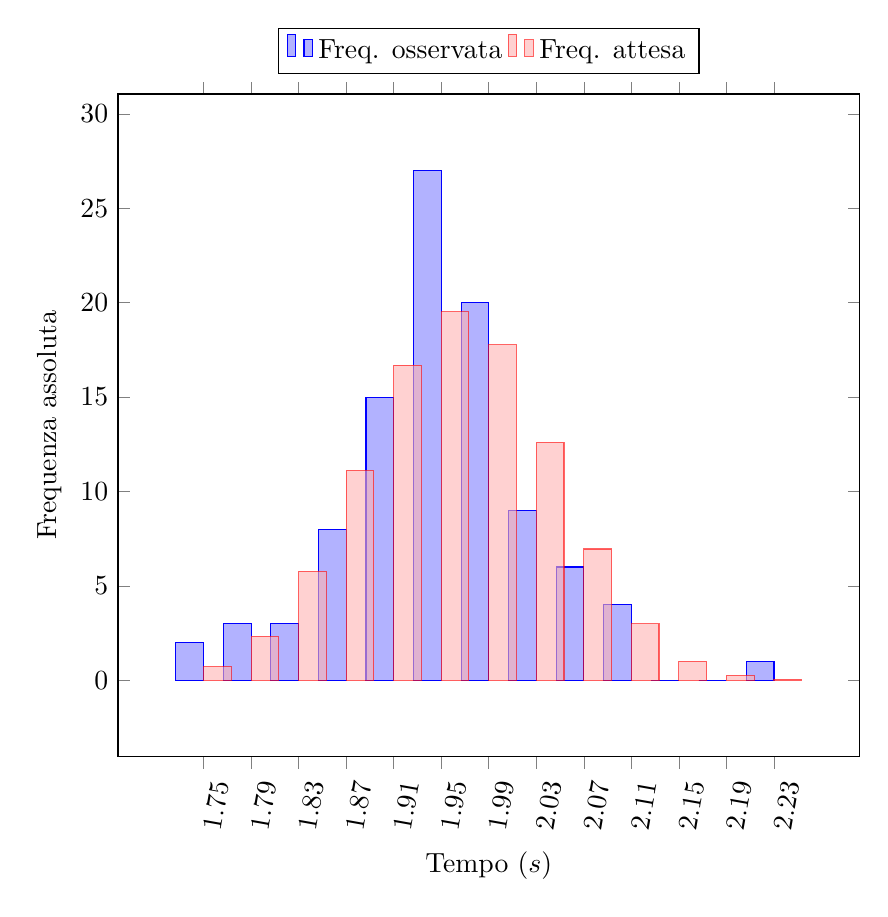
\begin{tikzpicture}
		\pgfplotsset{compat = 1.3}
		\begin{axis}[
			width=11cm, 
			height=10cm,
			ylabel=Frequenza assoluta,
			xlabel=Tempo $(s)$,
			enlargelimits=0.15,
			legend style={at={(0.5,1.1)},	anchor=north,legend columns=-1},
			ybar=0pt,% configures `bar shift'
			bar width=10pt,
			xtick={1.745,
				1.785,
				1.825,
				1.865,
				1.905,
				1.945,
				1.985,
				2.025,
				2.065,
				2.105,
				2.145,
				2.185,
				2.225},
			xticklabel style={rotate=80, anchor=north east}
			]
			\addplot+[opacity=1] 
			coordinates {
			(1.745,2)
			(1.785,3)
			(1.825,3)
			(1.865,8)
			(1.905,15)
			(1.945,27)
			(1.985,20)
			(2.025,9)
			(2.065,6)
			(2.105,4)
			(2.145,0)
			(2.185,0)
			(2.225,1)};
			\addplot+[opacity=0.6]
			coordinates {
			(1.745,0.733)
			(1.785,2.330)
			(1.825,5.767)
			(1.865,11.116)
			(1.905,16.688)
			(1.945,19.510)
			(1.985,17.764)
			(2.025,12.597)
			(2.065,6.957)
			(2.105,2.992)
			(2.145,1.002)
			(2.185,0.261)
			(2.225,0.053)
			};
			\legend{Freq. osservata,Freq. attesa}
		\end{axis}
	\end{tikzpicture}
	\end{center}
	\vspace{0.2cm}
	
	\paragraph{Ipotesi del test} La distribuzione teorica di Gauss si adatta alla distribuzione delle mie misure.
	\vspace{0.4cm}
	\begin{table}[H]
		\centering
		\begin{tabular}{lr}
			Livello di significatività 		& $ \quad 5\%$  \\
			Valore di $\chi ^2$             & $\quad 6.39$       \\
			Numero di gradi di libertà      & $\quad (7-2-1) = 4$         \\   
			Valore di $\chi ^2$ critico     & $\quad 9.48$
		\end{tabular}
	\end{table}
	 
	\newpage
	\section{Test di Gauss}
	Per verificare che il valor medio da me calcolato non si discosti significativamente dal valore misurato dalla fotocellula si utilizzerà il test Z, o test di Gauss. La mia stima del periodo del pendolo è $\bar{x} = 1.95s \pm 0.01 s$; il periodo calcolato dalla fotocellula è $ \mu = 1.957 \pm 0.001$. 
	
	Per prima cosa trovo quanto dista la mia migliore stima del periodo del pendolo dal valore misurato dalla fotocellula in unità della deviazione standard e lo assegno alla variabile $|z_{\text{oss}}|$:
	\[
	|z_{\text{oss}}| = \frac{\bar{x} - \mu}{\sigma}
	\]
	Mi chiedo quindi quale sia la probabilità di ottenere una discrepanza maggiore del mio $|z_{\text{oss}}|$, ovvero mi chiedo quale sia la probabilità di ricadere nelle code della curva.
	
	\noindent
	Per fare ciò cambiare variabile nella funzione così da ottenere una curva centrata in zero. \\
	
	\noindent
	Definisco una variabile $z = \frac{x-\mu}{\sigma}$:
	\[
	\frac{1}{\sqrt{2\pi}\sigma} \int_{-t}^{t}e^{-\frac{-z^2}{2}} \,dz
	\]
	
	Questa nuova espressione della curva gaussiana nella variabile standardizzata $z$ è centrata in $0$ ($\mu_z =0$) e ha deviazione standard = 1 ($\sigma_{z} = 1$).

\vspace{0.5cm}
\begin{center}
\begin{minipage}[l]{0.45\textwidth}
	\begin{tikzpicture}
		\begin{axis}[
			axis lines = middle,
			xlabel = \( x \),
			ylabel = \( f(x) \),
			ymin = 0,
			ymax = 1.2,
			xmin = -1,
			xmax = 5,
			xtick = {-1,0,1,2,3,4,5},
			xticklabels = { , , \(-\sigma\),,\(\sigma\), ,},
			yticklabel=\empty,
			domain = -1:5,
			samples = 100,
			smooth,
			every axis plot post/.append style={mark=none}
			]
			
			\addplot[blue, thick] {exp(-(x-2)^2)};
		\end{axis}
	\end{tikzpicture}	
\end{minipage}
\hspace{0.5cm}
\begin{minipage}[r]{0.45\textwidth}
	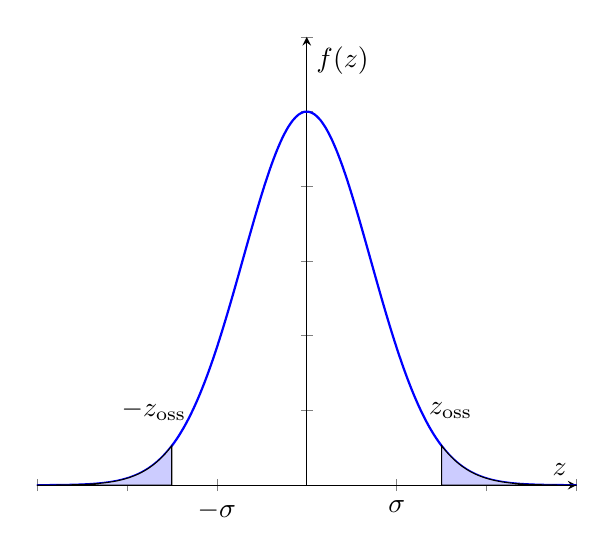
\begin{tikzpicture}
		\begin{axis}[
			axis lines = middle,
			xlabel = \( z \),
			ylabel = \( f(z) \),
			ymin = 0,
			ymax = 1.2,
			xmin = -3,
			xmax = 3,
			xtick = {-3,-2,-1,0,1,2,3},
			xticklabels = { , , \(-\sigma\), 0 ,\(\sigma\), ,},
			yticklabel=\empty,
			domain = -3:3,
			samples = 100,
			smooth,
			every axis plot post/.append style={mark=none}
			]
			
			\addplot[blue, thick] {exp(-x^2)};
			\addplot[fill=blue!20, domain=-3:-1.5] {exp(-x^2)} \closedcycle;
			\addplot[fill=blue!20, domain=1.5:3] {exp(-x^2)} \closedcycle;
			
			\node[] at (axis cs: -1.7, 0.2) {\( -z_{\text{oss}} \)};
			\node[] at (axis cs: 1.6, 0.2) {\( z_{\text{oss}} \)};
			
		\end{axis}
	\end{tikzpicture}	
\end{minipage}
\end{center}
	
	
	\paragraph{Ipotesi nulla $H_{0}$} La media della popolazione delle mie misure è uguale al valore misurato dalla fotocellula:
	\[
	\mu = 1.957s \pm 0.001 s
	\]
	
	\begin{table}[H]
		\centering
		\begin{tabular}{lr}
			Livello di significatività $\alpha$		& $ \quad 5\%$  \\
			Valore di $z$ critico     & $\quad 1.96$ \\
			Valore di $|z_{\text{oss}}|$      & $\quad 0.88$ \\
			p-value     & $\quad 0.38$
		\end{tabular}
	\end{table}

	
	

	\paragraph{Conclusione}  \colorbox{green}{\textbf{Accetto}} l'ipotesi nulla $H_{0}$ e concludo affermando che la mia stima è compatibile con il valore vero con un livello di significatività del $5\%$.
	
	
	
	\newpage
	\section{Punto 7}
	\newpage
	\section{Punto 8}
	
	\newpage
	\section{Punto 9}
	
	
	
\end{document}
